\section{Résultats}

\subsection{Résultats numériques}

Les grandeurs physiques ont pour unités celles du système international.

Les itérations sur la vitesse propulsive sont effectuées dans le script \lstinline+set_config.m+~: les problèmes d'étagement et de trajectoire sont résolus respectivement grâce aux fichiers \lstinline+stage_solver.m+ et \lstinline+path_solver.m+.

Voici les résultats issus de l'exécution du script principal~:

\[\begin{array}{|c|c|c|c|c|c|}\hline
\text{itérations} & \masspropel{} & \propellingvlct & \realvlct & \mathrm{M}_0 & \theta\\ \hline
2 & \begin{pmatrix}26\,841\\ 12\,496\\ 5\,491\end{pmatrix} & 9\,324 & 7\ 780,87 & 51\,984 & %
\begin{pmatrix}0,053\\ -0,137\,27\\ 0,327\,56\\ 0,139\,06\end{pmatrix}\\\hline
\end{array}\]

La vitesse cible $\targetvlct$ vaut dans notre cas $7\,784,26$.

\subsection{Graphes : trajectoire, altitude, vitesse et masse}

Voici les durées de combustion et instants $t_j$ de fin de combustion pour chaque étage~:

\[\begin{array}{|c|c|c|}\hline
\durcombustion{1} & \durcombustion{2} & \durcombustion{3}\\\hline
89,5 & 166,9 & 298,7\\\hline
\end{array}\]

\[\begin{array}{|c|c|c|}\hline
t_{1} & t_{2} & t_{3}\\\hline
\durcombustion{1} & 256,4 & 555,1\\\hline
\end{array}\]

\clearpage
\begin{center}
\begin{figure}[htbp]
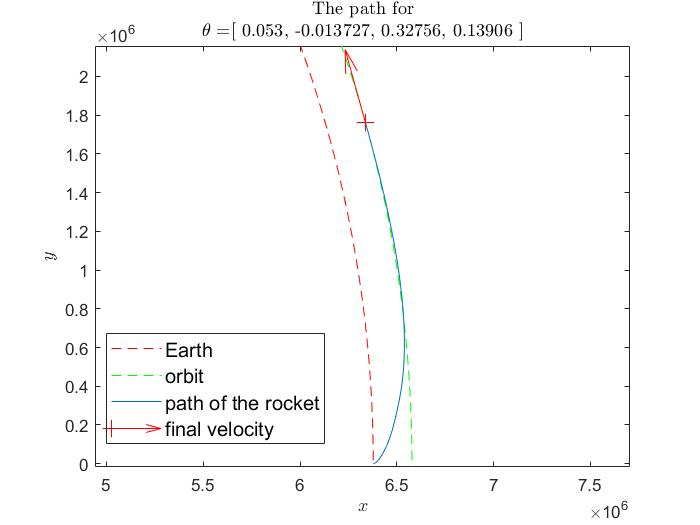
\includegraphics[scale=0.65]{./graphs/path.jpg}
\caption{trajectoire de la fusée et vecteur vitesse final}
\end{figure}
\end{center}

D'après ce graphe, il semble que l'altitude cible est atteinte et que le vecteur vitesse final est bien tangent à l'orbite visée.

\clearpage
\begin{center}
\begin{figure}[t]
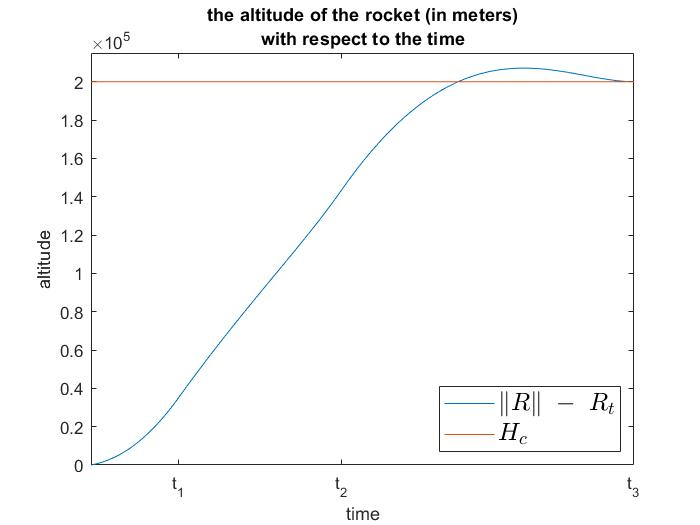
\includegraphics[scale=0.65]{./graphs/altitude.jpg}
\caption{altitude de la fusée en fonction du temps}
\end{figure}
\end{center}

L'altitude cible est bien atteinte selon ce graphe.

\clearpage
\begin{center}
\begin{figure}[t]
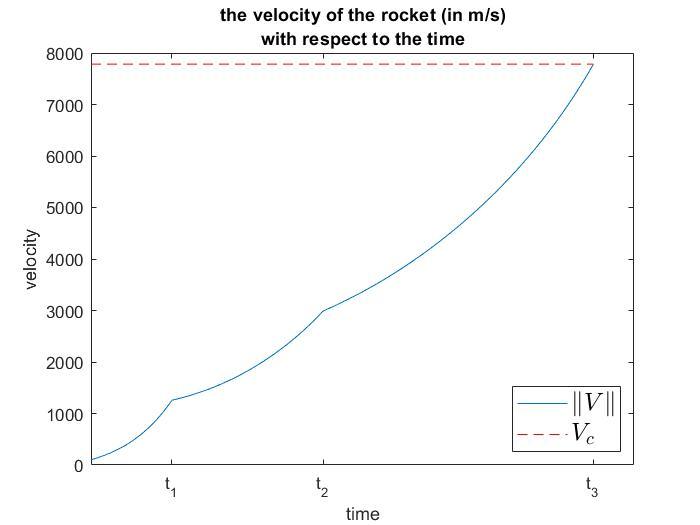
\includegraphics[scale=0.65]{./graphs/velocity.jpg}
\caption{vitesse de la fusée en fonction du temps}
\end{figure}
\end{center}

On peut s'assurer avec ce graphe que la vitesse cible est vraiment atteinte.

\clearpage
\begin{center}
\begin{figure}[t]
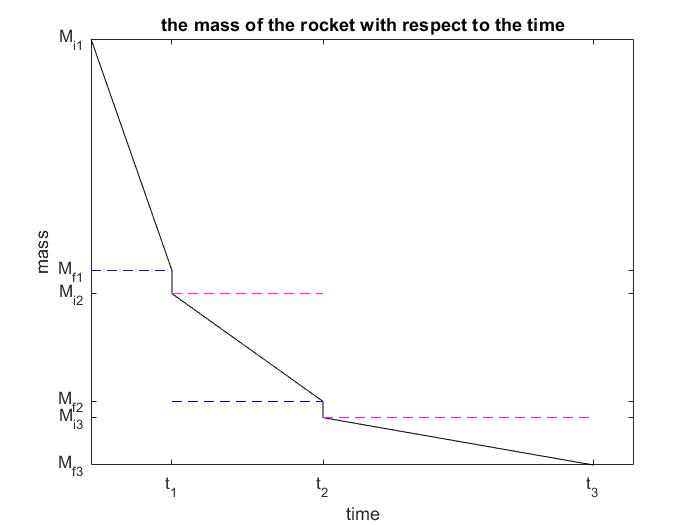
\includegraphics[scale=0.65]{./graphs/mass.jpg}
\caption{masse de la fusée en fonction du temps}
\end{figure}
\end{center}

La masse est bien une fonction affine par morceaux. La masse utile n'a pas été représentée afin de rendre le graphe plus clair.
